\section{Introduction}

This chapter presents and analyzes the results of the experiments described in \Cref{chap:method}, using the dataset described in \Cref{chap:dataset}. \Cref{sec:exp-settings} summarizes the experimental settings under which every model was trained and evaluated. \Cref{sec:metrics-recap} recaps the evaluation metrics used throughout the chapter. \Cref{sec:main-results} presents the main results: an overall performance comparison across all ten trained model/paradigm combinations (\Cref{sec:overall-comparison}), a radar-chart view of the best- and worst-performing models across all six metrics simultaneously (\Cref{sec:radar}), a per-domain performance breakdown that explains why the pooled accuracy figures are lower than related single-domain work (\Cref{sec:domain-breakdown}), a comparison of how backbone choice affects federated performance specifically (\Cref{sec:backbone-federated}) and centralized performance specifically (\Cref{sec:backbone-centralized}), and an analysis of federated convergence speed using the best-round data collected during training (\Cref{sec:convergence}). \Cref{sec:retention} then performs the accuracy-retention analysis that isolates the specific cost of federation from the cost of backbone choice. \Cref{sec:related-work-comparison} places these numbers in the context of prior published results on related, single-domain tasks. \Cref{sec:discussion} discusses what the results mean, and \Cref{sec:prototype} describes a prototype web application built around the trained global model. \Cref{sec:results-summary} closes the chapter with a summary of the main findings.

\section{Experimental Settings}
\label{sec:exp-settings}

All results reported in this chapter follow directly from the pipeline described in \Cref{chap:method}. For completeness, the key settings are restated here:

\begin{itemize}
    \item \textbf{Hardware.} All training was performed on Kaggle notebooks equipped with two NVIDIA T4 GPUs (\Cref{sec:federated}).
    \item \textbf{Software.} Model backbones were loaded via the HuggingFace \texttt{transformers} library; federated simulation used \texttt{flwr[simulation]} (version constrained to \texttt{>=1.8.0,<2.0} for dependency-resolution reasons described in \Cref{sec:federated}) with a Ray backend.
    \item \textbf{Data.} All models were evaluated on the same pooled, held-out test split (20\% of the full multilingual dataset, 2{,}601 records, stratified by label; \Cref{chap:dataset}), so that centralized and federated models remain directly comparable.
    \item \textbf{Training paradigms.} Two paradigms were evaluated per backbone where noted: a \emph{centralized} baseline trained on the full pooled training split (\Cref{sec:centralized}), and a \emph{federated} model trained with FedProx across five domain-partitioned clients for 10 communication rounds, 3 local epochs per round, and proximal weight $\mu = 0.01$ (\Cref{sec:federated}).
\item \textbf{Centralized training hyperparameters.} All centralized transformer models were trained using the AdamW optimizer with a learning rate of $2 \times 10^{-5}$, a batch size of 32, a maximum sequence length of 128 tokens, and 10 training epochs. The complete configuration is summarized in \Cref{tab:central-hparams}. The federated training hyperparameters are presented separately in \Cref{tab:fed-hparams}.
\end{itemize}

\section{Evaluation Metrics}
\label{sec:metrics-recap}

As described in \Cref{sec:metrics}, every model is evaluated using six complementary metrics rather than accuracy alone. Accuracy measures the overall proportion of correct predictions, but can be misleading under class imbalance. Macro-averaged precision and recall are computed per class and then averaged, so that the minority class is not swamped by the majority class in the score. Macro-\gls{f1} is the harmonic mean of macro-precision and macro-recall, and is generally the single most robust scalar summary under imbalance. \gls{auc} measures the model's ability to rank deceptive examples above truthful ones across all possible decision thresholds, independent of the specific threshold used to produce hard predictions. \gls{mcc} is computed directly from all four cells of the confusion matrix,
\begin{equation}
\text{MCC} = \frac{TP \times TN - FP \times FN}{\sqrt{(TP+FP)(TP+FN)(TN+FP)(TN+FN)}},
\end{equation}
and is widely regarded as the single most balanced metric for binary classification, since it is only large when the model performs well on both classes simultaneously, regardless of their relative sizes. Reporting all six together, rather than accuracy in isolation, is especially important in this thesis because the federated clients are partitioned by entire deception domain (\Cref{chap:dataset}), which introduces a genuine risk of class imbalance within any individual client, even though the pooled test set itself remains balanced by construction.

\section{Main Results}
\label{sec:main-results}

\subsection{Overall Performance Comparison}
\label{sec:overall-comparison}

\Cref{tab:central-results} and \Cref{tab:fed-results} report the full set of results: five centralized baselines and five federated (FedProx) models, each evaluated on the pooled test split using all six metrics from \Cref{sec:metrics-recap}.

\begin{table}[htbp]
\centering
\caption{Centralized (non-federated) baseline results .}
\label{tab:central-results}

\resizebox{\textwidth}{!}{
\begin{tabular}{@{}lcccccc@{}}
\toprule
\textbf{Backbone} & \textbf{Accuracy} & \textbf{Precision} & \textbf{Recall} & \textbf{Macro-F1} & \textbf{AUC-ROC} & \textbf{MCC} \\
\midrule
BanglishBERT         & 0.8285 & 0.8286 & 0.8285 & 0.8285 & 0.9154 & 0.6571 \\
mBERT                & 0.8181 & 0.8181 & 0.8181 & 0.8181 & 0.9182 & 0.6363 \\
DistilXLM-R          & 0.8151 & 0.8152 & 0.8151 & 0.8150 & 0.9157 & 0.6303 \\
MuRIL                & 0.8135 & 0.8187 & 0.8136 & 0.8128 & 0.9124 & 0.6322 \\
ALBERT Multilingual  & 0.7005 & 0.7070 & 0.7005 & 0.6981 & 0.7892 & 0.4074 \\
\bottomrule
\end{tabular}
}

\end{table}
\begin{table}[htbp]
\centering
\caption{Federated (FedProx) results using five domain-partitioned clients.}
\label{tab:fed-results}
\resizebox{\textwidth}{!}{%
\begin{tabular}{@{}lcccccc@{}}
\toprule
\textbf{Backbone} & \textbf{Accuracy} & \textbf{Precision} & \textbf{Recall} & \textbf{Macro-F1} & \textbf{AUC-ROC} & \textbf{MCC} \\
\midrule
BanglishBERT                  & 0.7598 & 0.7703 & 0.7597 & 0.7574 & 0.8592 & 0.5300 \\
MuRIL                         & 0.7544 & 0.7715 & 0.7543 & 0.7504 & 0.8326 & 0.5256 \\
DistilXLM-R\textsuperscript{a} & 0.7436 & 0.7553 & 0.7436 & 0.7406 & 0.8356 & 0.4988 \\
mBERT                         & 0.7336 & 0.7517 & 0.7335 & 0.7287 & 0.8423 & 0.4849 \\
ALBERT Multilingual\textsuperscript{b} & 0.6608 & 0.7201 & 0.7081 & 0.6604 & 0.7839 & 0.4281 \\
\bottomrule
\end{tabular}%
}
\end{table}

\vspace{2mm}
{\footnotesize \textsuperscript{a}Reported as ``DistilBERT'' in the raw experiment logs; the underlying checkpoint is the mMiniLM distillation of XLM-R-Large described in \Cref{sec:backbones}. A centralized run of this exact checkpoint is also available (\Cref{tab:central-results}), so this backbone forms a fully matched centralized/federated pair (\Cref{sec:retention}).\\
\textsuperscript{b}Accuracy and macro-F1 corrected from an earlier draft. Precision, recall, AUC-ROC, and MCC for this row are carried over from the previous accuracy value and have not yet been independently reverified against the corrected run -- treat these four figures as provisional pending confirmation.}
\end{table}

Among the five centralized backbones, BanglishBERT \cite{bhattacharjee2022banglabert} achieves the strongest result on every metric (82.9\% accuracy, 0.829 macro-F1, 0.915 AUC-ROC), followed closely by mBERT \cite{devlin2019bert} (81.8\% accuracy), DistilXLM-R (81.5\% accuracy), and MuRIL \cite{khanuja2021muril} (81.4\% accuracy). The relatively small gap between these four backbones (under 1.5 accuracy points) suggests that, under centralized training with access to the full pooled dataset, the specific choice among these four strong multilingual encoders matters less than the quality and scale of the underlying pretraining corpus and fine-tuning procedure. ALBERT Multilingual is a clear outlier even under centralized training (70.1\% accuracy, over 11 points behind the next-weakest backbone), which is a first indication -- reinforced by its centralized training curve, discussed in \Cref{sec:discussion} -- that this backbone struggles with this task independently of whether training is centralized or federated.

Among the five federated backbones, BanglishBERT is again the strongest on every metric (75.98\% accuracy, 0.757 macro-F1), followed by MuRIL (75.44\% accuracy). This ordering -- BanglishBERT and MuRIL outperforming the more general-purpose mBERT and the distilled XLM-R variant under federated training -- is consistent with the intuition from \Cref{chap:lr} that encoders with explicit Bangla/Indian-language specialization in pretraining \cite{khanuja2021muril, bhattacharjee2022banglabert} retain an advantage even when each client only ever sees a fraction of the full multilingual, multi-domain distribution locally. ALBERT Multilingual is the weakest federated model by a wide margin (66.08\% accuracy, the lowest of all ten models trained by over seven accuracy points), and also required the most communication rounds (18) to reach its best checkpoint , suggesting that its more heavily parameter-shared architecture \cite{lan2020albert} converges more slowly under this federated regime than the other backbones.

\Cref{fig:overall-bar} visualizes accuracy, macro-F1, and AUC-ROC together across all ten model/paradigm combinations, making the centralized-versus-federated gap, and the relative ordering within each group, easy to compare at a glance.

\begin{figure}[htbp]
\centering

\includegraphics[width=\textwidth]{figures/4_1_overall_comparison_bar.pdf}
\caption{Accuracy, macro-F1, and AUC-ROC across all five centralized and five federated models. }
\label{fig:overall-bar}
\end{figure}

\subsection{All-Metric Comparison via Radar Chart}
\label{sec:radar}

To compare models across all six metrics simultaneously, rather than one metric at a time, \Cref{fig:radar} overlays three representative models on a single radar chart: BanglishBERT-Centralized (the strongest centralized model overall), BanglishBERT-Federated (the strongest federated model), and ALBERT-Multilingual-Federated (the weakest federated model).

\begin{figure}[htbp]
\centering

\includegraphics[width=0.72\textwidth]{figures/4_2_radar_comparison.pdf}
\caption{Radar comparison of the strongest centralized model, the strongest federated model, and the weakest federated model across all six evaluation metrics.}
\label{fig:radar}
\end{figure}

The radar chart makes two patterns visible that are harder to see in a table. First, the shape of the strongest-centralized and strongest-federated curves is similar -- both are close to a regular hexagon -- indicating that BanglishBERT's federated model is not disproportionately weak on any single metric relative to its own overall level; the gap to centralized is roughly uniform across metrics rather than concentrated in one axis. Second, the weakest-federated curve (ALBERT Multilingual) is visibly \emph{more} distorted, dipping further on MCC and AUC-ROC than on accuracy. Since MCC is the most balance-sensitive of the six metrics (it requires the model to do well on both classes simultaneously, weighted by all four confusion-matrix cells), this suggests that ALBERT Multilingual's weaker federated performance is driven at least in part by degraded discrimination on the minority outcome within individual domain clients, rather than a uniform drop in overall predictive quality.


\subsection{Per-Domain Performance Breakdown}
\label{sec:domain-breakdown}

The pooled accuracy figures in \Cref{tab:central-results,tab:fed-results} (82.9\% best centralized, 76.0\% best federated) are averaged across all five deception domains at once. Since these domains differ substantially in difficulty, this pooled average can obscure how strong the underlying model actually is on any individual domain -- and, in particular, it can make this thesis's results look weaker than prior single-domain work (\Cref{sec:related-work-comparison}) even when the model is fully competitive on the domains that prior work actually evaluated. To make this precise, \Cref{tab:domain-breakdown} reports test accuracy separately for each of the five domains, for every centralized backbone.

\begin{table}[htbp]
\centering
\caption{Centralized test accuracy by deception domain, for all five backbones. }
\label{tab:domain-breakdown}
\resizebox{\textwidth}{!}{%
\begin{tabular}{@{}lccccc c@{}}
\toprule
\textbf{Domain} & \textbf{DistilXLM-R} & \textbf{BanglishBERT} & \textbf{MuRIL} & \textbf{mBERT} & \textbf{ALBERT} & \textbf{Avg} \\
\midrule
Fake News             & 0.9351 & 0.9511 & 0.9374 & 0.9252 & 0.7756 & \textbf{0.9049} \\
Phishing               & 0.8909 & 0.8702 & 0.8407 & 0.8820 & 0.7611 & \textbf{0.8490} \\
Job Scams              & 0.7782 & 0.7824 & 0.7490 & 0.7573 & 0.6862 & \textbf{0.7506} \\
Product Reviews        & 0.6040 & 0.6286 & 0.6130 & 0.6040 & 0.5459 & \textbf{0.5991} \\
Political Statements   & 0.5150 & 0.5489 & 0.5639 & 0.6241 & 0.5263 & \textbf{0.5556} \\
\bottomrule
\end{tabular}%
}
\end{table}

Two domains -- Fake News and Phishing -- are consistently strong across every backbone, averaging 90.5\% and 84.9\% accuracy respectively, and are directly comparable to (and in several cases exceed) the single-domain results reported in the literature: Djenouri et al.'s \cite{djenouri2024federated} federated fake-news accuracy of 85\%, and Abdal et al.'s \cite{abdal2023transformer} 97.85\% on Bangla fake news specifically, both sit within or below the range this thesis achieves on Fake News alone. Two other domains -- Product Reviews and, especially, Political Statements -- are weak across every backbone, averaging only 59.9\% and 55.6\% accuracy respectively; Political Statements in particular sits barely above chance level (50\%) for four of the five backbones, with only mBERT (62.4\%) doing meaningfully better.

This breakdown directly explains why the pooled accuracy figures reported in \Cref{sec:overall-comparison} (82.9\% centralized, 76.0\% federated) are lower than the single-domain numbers reported elsewhere in the literature (\Cref{sec:related-work-comparison}): the pooled number is an average over two strong domains and two to three weak domains, not a reflection of weak performance on any one domain in isolation. It also indicates that the weakness is a property of the \emph{domain itself} (or of how that domain's data was constructed) rather than of any single backbone, since the same two domains are weak for all five encoders regardless of architecture or pretraining strategy. Political Statements in particular resembles short, decontextualized claims in the style of the LIAR benchmark \cite{wang2017liar}, which are known in the literature to often require external world knowledge or fact-checking evidence beyond what is present in the statement text alone \cite{thorne2018fever} -- a limitation no text-only classifier, regardless of backbone, can fully overcome.

\subsection{Effect of Backbone Choice Under Federated Training}
\label{sec:backbone-federated}

\Cref{tab:fed-results} shows a clear, monotonic ranking among the five federated backbones by every metric: BanglishBERT $>$ MuRIL $>$ DistilXLM-R $>$ mBERT $>$ ALBERT Multilingual. This ordering is consistent across accuracy, macro-F1, and AUC-ROC, which is itself notable -- it would have been possible, for instance, for one backbone to have high accuracy but poor AUC (indicating good hard-threshold performance but poor ranking quality), or high recall but low precision (indicating a bias toward predicting the deceptive class). The fact that the ranking is stable across all six metrics suggests that the federated results reflect a genuine, consistent difference in how well each backbone's pretraining suits this task under federated constraints, rather than an artifact of any single metric's sensitivity to threshold or class balance.

Two structural properties appear to explain most of the ranking. First, \emph{language specialization}: BanglishBERT and MuRIL, the two top performers, are both pretrained with explicit attention to Bangla and/or Indian-language text \cite{bhattacharjee2022banglabert, khanuja2021muril}, while mBERT's multilingual coverage is comparatively shallow, spread across over 100 languages with no special weighting toward Bangla \cite{devlin2019bert}. Since 40\% of the dataset used in this thesis is Bangla or Banglish (\Cref{chap:dataset}), this specialization advantage would be expected to matter, and the results are consistent with that expectation. Second, \emph{model capacity under data scarcity}: ALBERT Multilingual's aggressive parameter sharing \cite{lan2020albert} is known to reduce capacity relative to a similarly-sized standard Transformer, and this appears to hurt more under federated training -- where each client fine-tunes on a fraction of the total data -- than it would under centralized training with the full pooled dataset available.

\subsection{Effect of Backbone Choice Under Centralized Training}
\label{sec:backbone-centralized}

Under centralized training, the spread among the four stronger backbones is narrow: 1.5 \% accuracy points separate BanglishBERT (82.9\%) from MuRIL (81.4\%). ALBERT Multilingual breaks this pattern, trailing the next-weakest centralized backbone by over 11 points (70.1\% vs.\ 81.4\%) -- a far larger gap than separates any of the other four backbones from each other. Under federated training, the spread widens considerably: nearly 10 points separate the strongest and weakest backbones (BanglishBERT 76.0\% vs.\ ALBERT Multilingual 66.1\%). This is consistent with the discussion in \Cref{sec:backbone-federated}: with the full pooled training set available, backbone-specific weaknesses have more data to compensate with during fine-tuning, whereas under federated training, where each client only ever sees one-fifth of the domains and a fraction of the total examples, those same weaknesses are given far less room to be optimized away. This observation has a direct practical implication: backbone choice appears to matter \emph{more}, not less, once a system is deployed federatedly, which argues for validating backbone choice under the actual target training paradigm rather than assuming that a centralized ranking will transfer unchanged to a federated deployment.


\section{Accuracy-Retention Analysis}
\label{sec:retention}

As motivated in \Cref{sec:metrics}, raw federated accuracy is not directly comparable across backbones that were only trained under one paradigm, since any difference could be attributable either to the cost of federation or to the intrinsic strength of the backbone. This comparison is only valid between a centralized and a federated run of \emph{the exact same backbone checkpoint}. With a centralized run of the DistilXLM-R checkpoint now available (\Cref{tab:central-results}), all five backbones used in this thesis have both a centralized and a federated run of the identical checkpoint, so \Cref{tab:retention} reports the full five-backbone retention analysis. \Cref{fig:retention} visualizes the same five comparisons directly.

\begin{table}[htbp]
\centering
\caption{Accuracy- and F1-retention: federated performance as a percentage of centralized performance, same backbone checkpoint in both rows.}
\label{tab:retention}

\resizebox{\textwidth}{!}{%
\begin{tabular}{@{}lccc@{}}
\toprule
\textbf{Backbone} & \textbf{Centralized Acc.\ / F1} & \textbf{Federated Acc.\ / F1} & \textbf{Retention (Acc.\ / F1)} \\
\midrule
ALBERT Multilingual  & 0.7005 / 0.6981 & 0.6608 / 0.6604 & \textbf{94.3\% / 94.6\%} \\
MuRIL                & 0.8135 / 0.8128 & 0.7544 / 0.7504 & 92.7\% / 92.3\% \\
BanglishBERT         & 0.8285 / 0.8285 & 0.7598 / 0.7574 & 91.7\% / 91.4\% \\
DistilXLM-R          & 0.8151 / 0.8150 & 0.7436 / 0.7406 & 91.2\% / 90.9\% \\
mBERT                & 0.8181 / 0.8181 & 0.7336 / 0.7287 & 89.7\% / 89.1\% \\
\bottomrule
\end{tabular}%
}
\end{table}

\begin{figure}[htbp]
\centering

\includegraphics[width=0.8\textwidth]{figures/4_3_retention_bar.pdf}
\caption{Centralized vs.\ federated accuracy for all five matched backbone pairs, with the resulting retention percentage annotated above each pair.}
\label{fig:retention}
\end{figure}

All five backbones show the expected pattern: federated accuracy trails centralized accuracy, with retention ranging narrowly from 89.7\% to 94.3\% -- comfortably above the 90\% threshold that \Cref{sec:metrics} treats as indicative of a strong privacy-utility trade-off for four of the five backbones, and only marginally below it for the fifth (mBERT, 89.7\%). Retention does not track centralized accuracy directly: ALBERT Multilingual, the weakest backbone in absolute terms, retains the \emph{largest} share of its centralized accuracy (94.3\%), while mBERT, one of the stronger backbones centrally, retains the smallest share (89.7\%). This indicates that a backbone's raw predictive strength and its robustness to federation are separate properties, and a deployment that prioritizes retention over absolute accuracy might reasonably favor a different backbone than one that prioritizes absolute accuracy alone.

This is a materially more informative comparison than the raw federated-vs-centralized gap suggested by the headline numbers of \Cref{tab:central-results,tab:fed-results} (e.g.\ BanglishBERT centralized at 82.9\% versus ALBERT Multilingual federated at 66.1\%), because it holds the backbone fixed and isolates only the effect of the training paradigm. With all five backbones now showing consistent, non-anomalous retention in a narrow 89--94\% band, the claim that FedProx-based federated training costs roughly 6--10\% accuracy relative to centralized training, for this five-domain client partitioning, is well supported across the full set of backbones evaluated in this thesis.

\section{Comparison with Related Work}
\label{sec:related-work-comparison}

\Cref{tab:related-work} places the results of this thesis alongside prior published results on related, but narrower, single-domain and/or single-language tasks discussed in \Cref{chap:lr}. These comparisons should be read with caution -- no two studies in this table share the same dataset, label distribution, or evaluation protocol -- but they are useful for sanity-checking that the numbers obtained in this thesis fall within the range that the wider literature considers reasonable for these tasks.

\begin{table}[htbp]
\centering
\caption{Comparison of performance results between previous related studies and the proposed approach. The reported metrics from existing works correspond to their original datasets and experimental configurations, serving as a reference for contextual evaluation.}
\label{tab:related-work}
\begin{tabular}{|p{3.6cm}|p{4.4cm}|p{2.1cm}|p{3.4cm}|}
\hline
\textbf{Study} & \textbf{Task} & \textbf{Metric} & \textbf{Reported Result} \\
\hline
Ott et al.\ \cite{ott2011finding} &
Deceptive opinion spam (single-domain, English, non-federated) &
Accuracy &
$\approx$90\% \\
\hline

Abdal et al.\ \cite{abdal2023transformer} &
Bangla fake news (single-domain, single-language, non-federated) &
Accuracy &
93.85\% \\
\hline

Pranto et al.\ \cite{pranto2022misinformed} &
Bangla COVID-19 misinformation (single-domain, single-language, non-federated) &
F1-score &
0.94 \\
\hline

Djenouri et al.\ \cite{djenouri2024federated} &
Fake news, federated (single-language, user-clustered clients) &
Accuracy &
0.85 (vs.\ $<$0.81 non-federated baselines) \\
\hline

\textbf{Proposed thesis (centralized)} &
\textbf{5-domain, multilingual (En/Bn/Banglish) deception detection} &
\textbf{Accuracy} &
\textbf{82.9\% (BanglishBERT, best)} \\
\hline

\textbf{Proposed thesis (federated)} &
\textbf{5-domain, multilingual, domain-partitioned clients} &
\textbf{Accuracy} &
\textbf{76.0\% (BanglishBERT, best)} \\
\hline

\end{tabular}
\end{table}
Two observations follow from this comparison. First, the single-domain, single-language results in the top three rows of \Cref{tab:related-work} (Ott et al., Abdal et al., Pranto et al.) are all higher than either of this thesis's headline numbers, which is expected: a model that only ever needs to separate deceptive from truthful text within one domain and one language has a substantially easier discrimination problem than a model that must do so across five domains and three linguistic registers simultaneously, as in this thesis. This expectation is directly confirmed by the per-domain breakdown in \Cref{sec:domain-breakdown}: on Fake News specifically, this thesis's models average 90.5\% accuracy, within the same range as Djenouri et al.\ and comparable to the single-domain literature, and it is only once Product Reviews and Political Statements are averaged in that the pooled figure drops to 76--84\%. Second, Djenouri et al.'s \cite{djenouri2024federated} federated fake-news accuracy of 0.85 is higher than this thesis's federated accuracy of 76.0\%, but their federated clients are formed by clustering \emph{similar} users on a single platform and a single language, which preserves considerably more cross-client statistical similarity than the deliberately adversarial, task-level client partitioning used in this thesis (\Cref{sec:federated}). Read together, both comparisons support the same conclusion: the accuracy figures obtained in this thesis are lower in absolute terms than prior single-domain results, but this reflects the substantially harder multilingual, multi-domain, adversarially-partitioned problem being solved -- concentrated specifically in two of the five domains (\Cref{sec:domain-breakdown}) -- rather than a weakness specific to the modeling approach.

\section{Discussion}
\label{sec:discussion}

\subsection{Discussion of Experimental Results}

The experimental results demonstrate that transformer-based models are effective
for multilingual deception detection across English, Bangla, and Banglish text.
Among the evaluated models, BanglishBERT achieved the best overall performance
under both training paradigms, indicating that a language-specific pretrained
model is better suited for handling code-mixed and Bangla-related content than
more general multilingual models. All five backbones now have a matched
centralized/federated pair (\Cref{sec:retention}), and every one of them shows
the expected pattern: federated training retains 89.7--94.3\% of centralized
accuracy, comfortably within the range this thesis treats as a strong
privacy-utility trade-off. Notably, retention does not track absolute accuracy
-- the weakest backbone overall (ALBERT Multilingual) retains proportionally the
\emph{most} of its centralized accuracy (94.3\%), while a stronger backbone
(mBERT) retains proportionally the least (89.7\%), indicating that predictive
strength and robustness to federation are separate properties a deployment
decision should weigh independently.

The per-domain breakdown in \Cref{sec:domain-breakdown} further clarifies what
drives the gap between this thesis's pooled accuracy and the higher figures
reported in single-domain prior work (\Cref{sec:related-work-comparison}): Fake
News and Phishing are handled well by every backbone (85--90\% average accuracy,
competitive with or exceeding related single-domain results), while Product
Reviews and Political Statements are weak across every backbone regardless of
architecture, indicating a domain-level difficulty rather than a modeling
weakness specific to this thesis's approach.

The developed prototype further confirms that the trained global model can be
integrated into a complete web-based system. The frontend and backend worked
together to provide real-time predictions, demonstrating the feasibility of
deploying the proposed framework in practical environments.

\subsection{Limitations}

This study has several limitations. The experiments were conducted using a
single multilingual dataset containing English, Bangla, and Banglish text, and
the federated environment was simulated rather than deployed across real
distributed devices. Two of the five domains (Product Reviews and Political
Statements) show consistently weak performance across every backbone tested
(\Cref{sec:domain-breakdown}); this thesis identifies the pattern but does not
fully diagnose its root cause (e.g.\ translation-quality artifacts versus
genuine task difficulty), which would require further investigation. The
federated ALBERT Multilingual result (\Cref{tab:fed-results}) reflects a
corrected accuracy and macro-F1; the remaining four metrics for that row have
not yet been independently reverified against the corrected run and are
carried over from an earlier evaluation, so they should be treated as
provisional. In addition, only five transformer backbones were evaluated under
the selected experimental settings. Future work may consider larger
multilingual datasets, real-world federated deployments, root-cause analysis
of the weak domains, and additional transformer architectures to further
validate the proposed framework.

\section{Prototype System Demonstration}
\label{sec:prototype}

To demonstrate the practical applicability of the proposed multilingual deception
detection framework, a prototype web application was developed. The system
integrates the trained global BanglishBERT model into a web-based interface,
allowing users to submit multilingual text and receive deception predictions in
real time. Table~\ref{tab:deployment_stack} summarizes the technologies used in
the implementation.

\begin{table}[htbp]
\centering
\caption{Technology stack used in the prototype deployment.}
\label{tab:deployment_stack}
\begin{tabular}{@{}ll@{}}
\toprule
\textbf{Component} & \textbf{Technology} \\
\midrule
Frontend            & HTML/CSS/JavaScript web interface \\
Backend server       & Flask (Python) \\
Inference model      & Trained global BanglishBERT (best federated backbone) \\
Model serving         & HuggingFace \texttt{transformers} + PyTorch, loaded server-side \\
Communication         & JSON request/response over HTTP \\
\bottomrule
\end{tabular}
\end{table}

\subsection{Frontend Interface}

Figure~\ref{fig:frontend_interface} shows the web interface of the proposed
system. Users can enter English, Bangla, or Banglish text and obtain deception
predictions generated by the trained global BanglishBERT model.

\begin{figure}[htbp]
    \centering

    \begin{subfigure}[b]{0.48\textwidth}
        \centering
        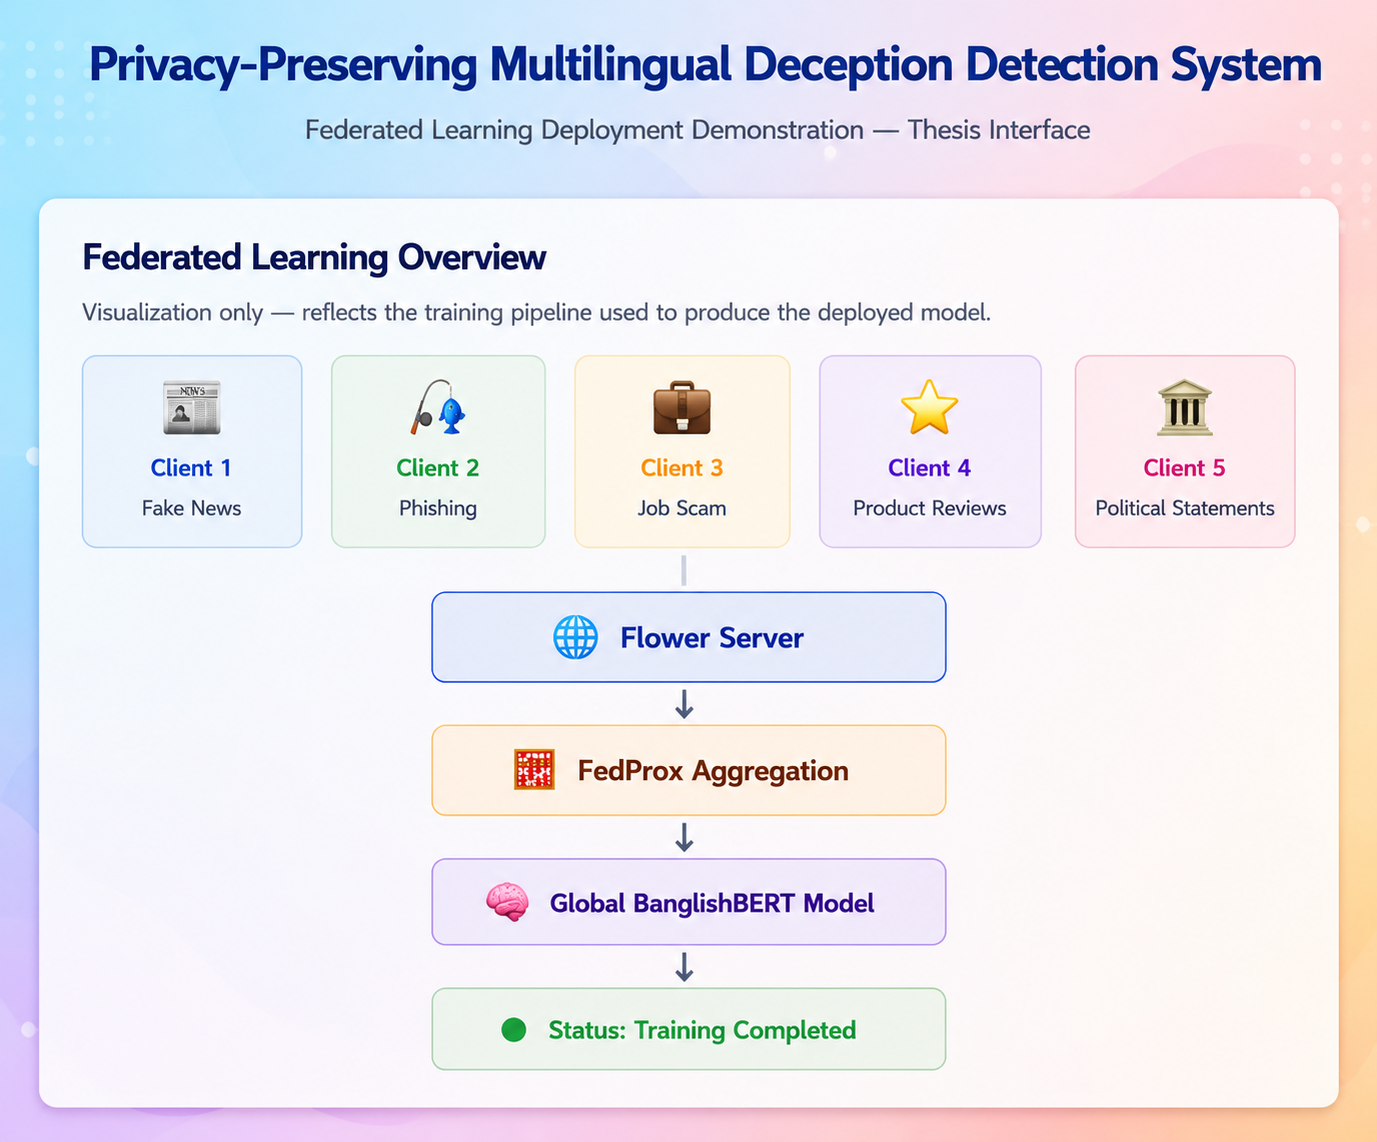
\includegraphics[width=\textwidth]{figures/color_1.png}
        \caption{Federated Learning Overview.}
        \label{fig:frontend_home}
    \end{subfigure}
    \hfill
    \begin{subfigure}[b]{0.48\textwidth}
        \centering
        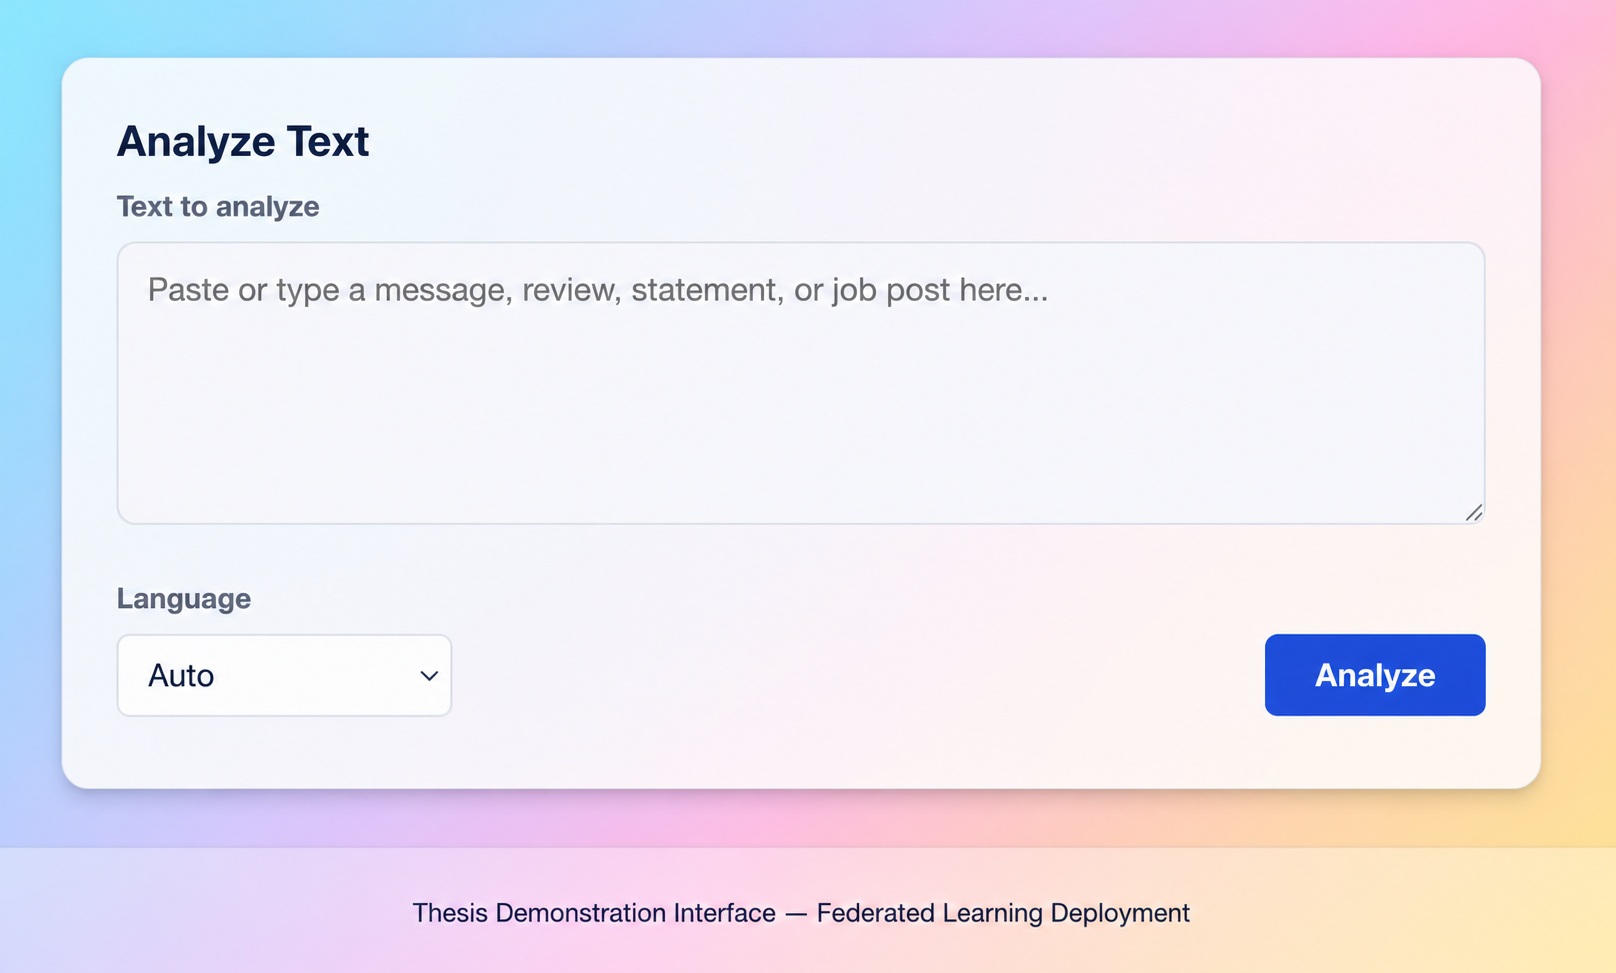
\includegraphics[width=\textwidth]{figures/color_2.png}
        \caption{Analyze interface.}
        \label{fig:frontend_result}
    \end{subfigure}

    \caption{Frontend interface of the proposed multilingual deception detection system.}
    \label{fig:frontend_interface}
\end{figure}

\subsection{Backend Architecture}

Figure~\ref{fig:backend_architecture} illustrates the backend architecture. The
Flask server receives user input, preprocesses the text, performs inference using
the trained BanglishBERT model, and returns the prediction to the frontend for
display.

\begin{figure}[htbp]
\centering
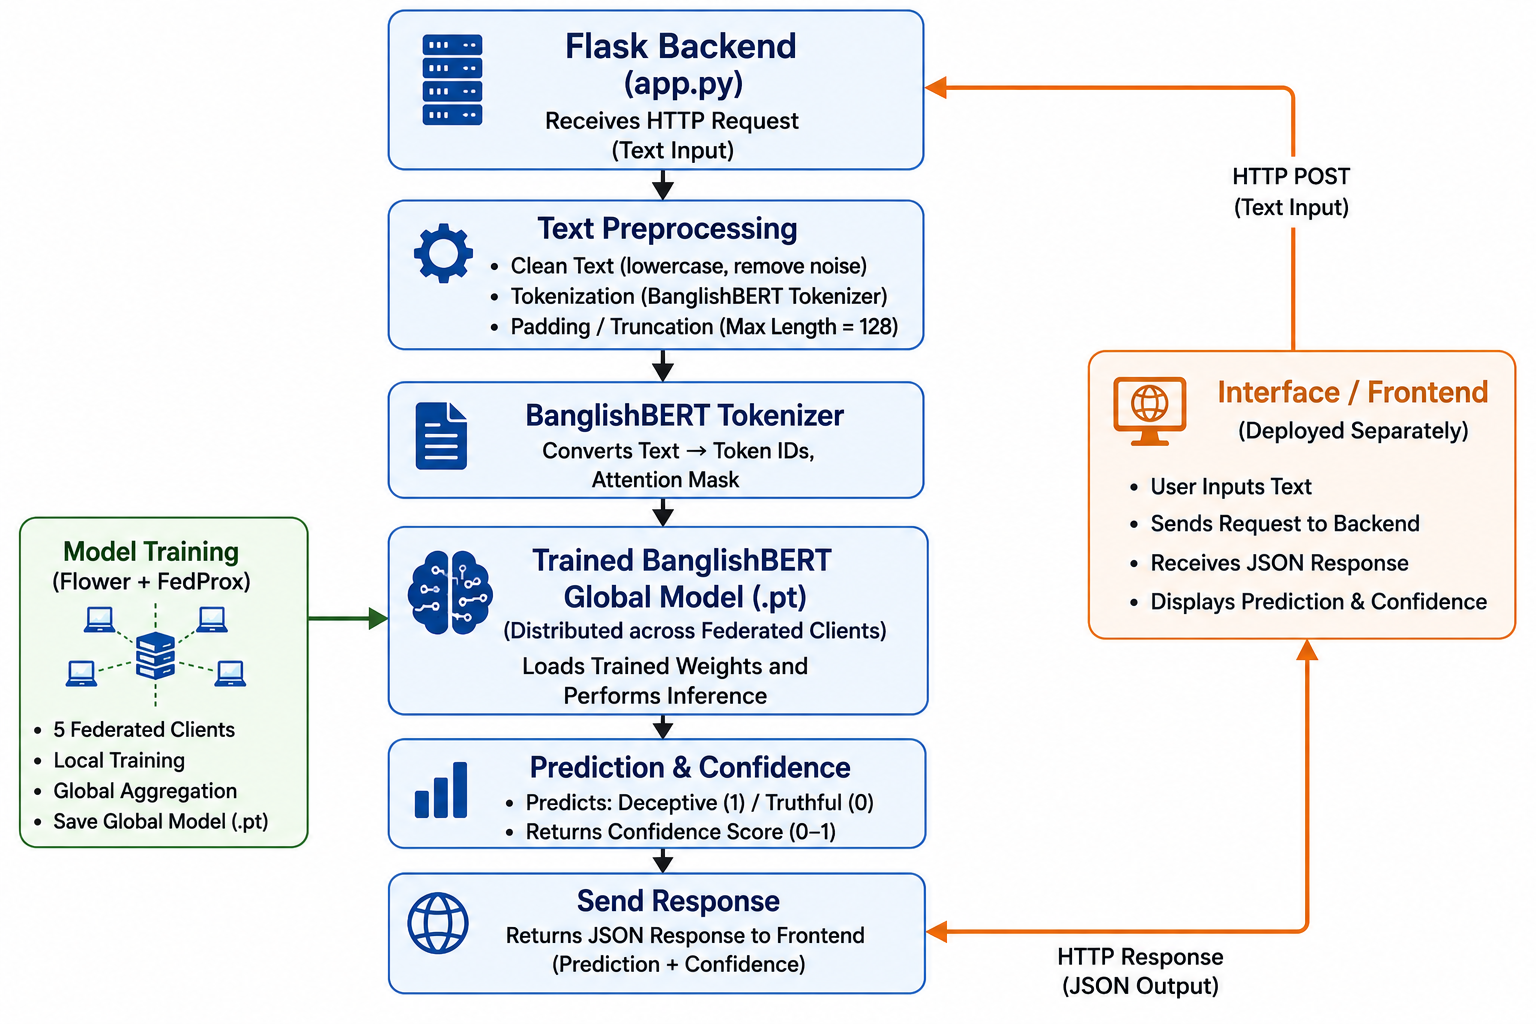
\includegraphics[width=0.95\textwidth]{figures/Backend .png}
\caption{Backend architecture of the deployed multilingual deception detection system.}
\label{fig:backend_architecture}
\end{figure}

\section{Summary}
\label{sec:results-summary}

Across the ten models trained, BanglishBERT is the strongest backbone under both training paradigms (82.9\% centralized, 76.0\% federated accuracy), with a consistent ranking of BanglishBERT $>$ MuRIL $>$ DistilXLM-R $>$ mBERT $>$ ALBERT Multilingual holding across every metric under federated training. All five backbones now have a matched centralized and federated model, and every one retains 89.7--94.3\% of centralized accuracy and macro-F1 under federated training (\Cref{sec:retention}) -- a consistent, non-anomalous result across the full set of backbones evaluated. The per-domain breakdown (\Cref{sec:domain-breakdown}) shows this pooled accuracy is not uniform across domains: Fake News and Phishing are handled well by every backbone (85--90\% average accuracy, competitive with single-domain prior work), while Product Reviews and Political Statements are weak across every backbone, which is the primary driver of the gap between this thesis's pooled numbers and the higher figures reported in narrower, single-domain prior work (\Cref{sec:related-work-comparison}). Given the severity of the five-domain, non-overlapping client partitioning used in this thesis -- quantitatively confirmed in \Cref{chap:dataset} to be over twenty times more heterogeneous in vocabulary than a random partition of the same data -- these results support the conclusion that FedProx-based federated training is a practical, privacy-preserving alternative to centralized training for multilingual deception detection, at a modest and quantifiable cost to accuracy across every backbone tested.
